\documentclass[conference]{IEEEtran}
\IEEEoverridecommandlockouts

\usepackage{cite}
\usepackage[portuguese,brazil]{babel}
\usepackage{amsmath, amssymb, amsfonts}
\usepackage[utf8]{inputenc}
\usepackage{algorithmic}
\usepackage{graphicx}
\usepackage{textcomp}
\usepackage{subfig}
\usepackage{diagbox}
\usepackage{ctable}
\def\BibTeX{{\rm B\kern-.05em{\sc i\kern-.025em b}\kern-.08em
    T\kern-.1667em\lower.7ex\hbox{E}\kern-.125emX}}
\begin{document}

\title{MO444 - Machine Learning - Relatório da Atividade \#2 Grupo 12}

\author{\IEEEauthorblockN{Bárbara Caroline Benato}
\IEEEauthorblockA{
RA 192865\\
barbarabenato@gmail.com}
\and
\IEEEauthorblockN{Breno Leite}
\IEEEauthorblockA{
RA 192863\\
brenolleite@gmail.com}}

\maketitle

\section{Introdução}

A segunda atividade da disciplina de \textit{Machine Learning} (MO444) tem como objetivo explorar técnicas de classificação de padrões multiclasse, a fim de se encontrar um sistema de detecção de objetos que faça o reconhecimento e classificação das imagens presentes na base de dados \textit{Cifar-10}. Assim, a solução apropriada deve ser encontrada evitando o supertreinamento dos dados. 

O objetivo deste relatório é apresentar os experimentos que foram desenvolvidos com intuito de encontrar o melhor modelo para classificar objetos presentes na base, utilizando a Regressão Logística e Rede Neural.

O mesmo é dividido em Seções. Na Seção \ref{sec:meto}, alguns dados interessantes sobre a base de dados são mostrados, bem como a metodologia empregada e as atividades desenvolvidas. Por fim,  a Seção \ref{sec:exp} apresenta os experimentos e as conclusões do trabalho.

\section{Materiais e Métodos} \label{sec:meto}

Os materiais, como a base de dados e pacote utilizados, e a metodologia empregados no presente trabalho são descritos a seguir.

\subsection{Base de dados \textit{Cifar-10}} \label{sec:base}

A base de dados \emph{Cifar-10} é utilizada para a validação dos estudos e objetivos propostos para o presente trabalho. A base de dados apresenta imagens de diferentes objetos, bem como o rótulo de cada objeto. O rótulo das imagens de objetos estão dividos em 10 classes, como, por exemplo, avião, carro, ave, gato, veado, cachorro, sapo, cavalo, barco e caminhão. A base de dados apresenta $60.000$ imagens coloridas de tamanho $32 \times 32$ \textit{pixels}, que são  divididas em $50.000$ imagens de treinamento e $10.000$ imagens para teste.

\subsection{Pacote \textit{Scikit-Learn}} \label{sec:pac}

Os modelos desenvolvidos para a Regressão Logística foram implementados utilizando funções do pacote \emph{Scikit-Learn}, em linguagem de programação \emph{Python}. A função \emph{LogisticRegression} foi empregada a fim de se obter uma solução base de Regressão Logística, bem como para Regressão Logística Multinomial.

A configuração dos parâmetros da função \emph{LogisticRegression} foi dada da seguinte forma:
\begin{itemize}
	\footnotesize \item \textit{penalty}: Uma penalidade que utiliza uma constante de regularização \footnotesize \textit{l2} é utilizada para obter uma solução esparsa.
	\footnotesize \item \textit{dual}: Falso, uma formulação primária é utilizada devido ao número de amostras ser maior que o número de características.
	\footnotesize \item \textit{tol}: Valor de tolerância utilizado como critério de parada de $0.0001$.
	\footnotesize \item \textit{C}: Valor responsável por controlar a força da regularização adicionada atribuído como $1$.
	\footnotesize \item \textit{fit\_intercept}: Verdadeiro, ou seja, a intersecção com o eixo y é calculada.
	\footnotesize \item \textit{intercept\_scaling}: Falso, pois é incompatível com o algoritmo de otimização escolhido.
	\footnotesize \item \textit{class\_weight}: Nenhum tipo de balanceamento, uma vez que o conjunto de dados é balanceado.
	\footnotesize \item \textit{random\_state}: Nenhum tipo de randomização é adicionada, pois é incompatível com o algoritmo de otimização escolhido.
	\footnotesize \item \textit{solver}: Algoritmo de otimização escolhido definido como \textit{lbfgs}, apropriado para o problema multiclasse.
	\footnotesize \item \textit{max\_iter}: Número máximo de iterações definido como $50$.
	\footnotesize \item \textit{multi\_class}: Parâmetro que define se o problema deve ser encarado como \textit{one vs rest} ou \textit{multinomial}. A documentação do pacote define o problema \textit{one vs all} com mesmo parâmetro para o problema \textit{one vs rest}. Ambos os parâmetros são abordados no presente trabalho. 
	\footnotesize \item \textit{warm\_start}: Falso, não se utiliza coeficientes obtidos anteriormente.
\end{itemize}


\subsection{Biblioteca \textit{Keras}} \label{sec:bib}

Já para os modelos desenvolvidos considerando Rede Neural, uma biblioteca de interface de desenvolvimento em alto nível de redes neurais foi utilizada\footnote{https://keras.io/}. Tal biblioteca é escrita em \emph{Python}. Optou-se por utilizar como base do \textit{Keras}, a biblioteca \textit{Theano} e a biblioteca \textit{TensorFlow}, que são bibliotecas que executam expressões matemáticas envolvendo vetores de muitas dimensões eficientemente. Ambas as bibliotecas foram escolhidas por apresentarem suporte ao processamento gráfico em GPUs e alcançar um maior aproveitamento dos experimentos em relação ao tempo de processamento, bem como os resultados encontrados.

A principal função utilizada para as camadas da Rede Neural é denominada \textit{Dense}. Tal função é capaz de representar redes neurais multicamadas totalmente conectada. A configuração de parâmetros é dada como segue:

\begin{itemize}
	\footnotesize \item \textit{units}: Dimensão da saída de cada camada definida como $3800$.
	\footnotesize \item \textit{activation}: Funções de ativação empregadas nos experimentos: linear, tangente hiperbólica, sigmoidal, relu e softmax. 
	\footnotesize \item \textit{use\_bias}: Verdadeiro, o vetor de bias é utilizado.
	\footnotesize \item \textit{kernel\_initializer}: Inicialização das matrizes de pesos utiliza inicialização uniforme Glorot, definida como padrão.
	\footnotesize \item \textit{bias\_initializer}: Bias inicializados com $0$.
	\footnotesize \item \textit{kernel\_regularizer}: Nenhuma função de regularização aplicada `as matrizes de peso.
	\footnotesize \item \textit{bias\_regularizer}: Nenhuma função de regularização aplicada ao vetor de bias.
	\footnotesize \item \textit{activity\_regularizer}:Nenhuma função de regularização aplicada `a saída da camada.
	\footnotesize \item \textit{kernel\_constraint}: Nenhuma constante de regularização aplicada `as matrizes de peso.
	\footnotesize \item \textit{bias\_constraint}: Nenhuma constante de regularização aplicada ao vetor de bias.
\end{itemize}

\subsection{Metodologia} \label{sec:met}

Um processo gradual foi abordado para solucionar o problema proposto neste trabalho, a partir de um modelo de menor complexidade para um modelo de maior complexidade. Primeiramente a técnica Regressão Logística foi aplicada utilizando a abordagem \emph{one-vs-all} para considerar o problema multiclasse. Em sequência um modelo de Regressão Lo Multinomial foi implementado, esses modelos foram utilizados como \emph{baseline} para o trabalho.

Com intuito de melhorar os resultados, redes neurais foram utilizadas. Diversos experimentos foram executados para encontrar a melhor configuração da rede. A principal métrica utilizada nos experimentos foi a acurácia, que mede em porcentagem a quantidade de acertos na classificação. A Tabela~\ref{tab:config} mostra as GPUs utilizados para os testes realizados nesse trabalho.


% comando nvidia-smi voce consegue ver (vc provavelmente sabe, mas se precisar ta aqui)
\begin{table}[h!]
	\centering
	\begin{tabular}{ll} \toprule
		  \textbf{GPU} & \textbf{GPU Memory} \\ \toprule 	
		  GeForce GTX 980 & 4043 MiB \\ 
		  GeForce GTX 1060 & 6072 MiB \\ 
		 \bottomrule
	\end{tabular}
	\caption{Configuração das placas de vídeo utilizadas nos experimentos.}
	\label{tab:config}
\end{table}

Os experimentos do trabalho estão divididos da seguinte forma: 

\begin{itemize}
	\item \textbf{Comparação entre regressão logística multinomial e utilizando a técnica \emph{one-vs-all}:} Neste experimento é realizada uma comparação entre a regressão logística utilizando a técnica \emph{one-vs-all} e a regressão logística multinomial, ambas utilizam os mesmos parâmetros. O objetivo desse experimento é encontrar um\emph{baselines}, a configuração de parâmetros não foi muito explorada.
	
	\item \textbf{Comparação entre diferentes modelos de redes neurais:} Para esta etapa, o objetivo é analisar diferentes modelos para as redes neurais, utilizando diferentes funções de ativação e números de camadas.  
	
	\item \textbf{Resultados dos melhores modelos na base de teste:} Por fim, os melhores modelos encontrados na etapa anterior são aplicados na base de testes com intuito de provar e mostrar a sua robustez.
\end{itemize}

\section{Experimentos e Discussões} \label{sec:exp}

Esta seção tem como objetivo mostrar os resultados obtidos pelos modelos desenvolvidos neste trabalho, assim como explicar os diversos experimentos realizados para a escolha do modelo final. Todos os experimentos desse trabalho utilizaram o processo de validação considerando $5$-\emph{folds} para o processo de treinamento. 

Como etapa de pré-processamento das imagens da base de dados, algumas técnicas foram consideradas e a biblioteca \emph{Scikit-Learn} foi utilizada. Primeiramente, os dados foram normalizados. Observou-se que a normalização padrão da biblioteca apresentava resultados diferentes comparada com a normalização que utilizava uma constante de regularização $l2$. Comparando a acurácia no conjunto de treinamento e de validação do modelo de redes neurais, observou-se que a normalização original apresentava alta taxa de acurácia de treinamento e baixa acurácia de validação e, ainda, que a diferença entre tais acurácias era reduzida quando utilizava-se a constante $l2$. Assim, o \emph{overfitting} dos dados pôde ser reduzido nesta etapa.

Após a normalização, os dados foram escalados utilizando a média dos dados. Considerando que a dimensão do problema, ou seja, o tamanho das imagens vetorizadas, é de $3.072$, tentou-se reduzir a dimensionalidade do problema.  A técnica \emph{Principal Component Analysis} (PCA) foi empregada considerando os valores de componentes principais de $2.000$, $1.000$, $500$, $300$ e $200$, e para nenhum dos valores o modelo apresentou alguma melhora na taxa de acerto. Observou-se, então que a redução de dimensionalidade não foi relevante para o problema para os valores de componentes principais escolhidos. Com o intuito de ressaltar as informações de contorno dos objetos, o filtro de Sobel foi aplicado. O filtro de Sobel, no entanto, não apresentou uma melhora, quanto a acurácia dos resultados. Acredita-se que a informação de cor deveria ser considerada ao problema e um descritor combinado poderia ter sido empregado. Como o objetivo da presente atividade não era explorar as técnicas para extração de características, o descritor combinado não foi implementado.

Assim, todos os experimentos consideraram a normalização utilizando a constante $l2$, bem como empregaram a escalabilidade dos dados com a informação da média.


\subsection{Baselime: Regressão Logística}

Esta seção mostra os resultados dos modelos de regressão logística utilizados como \emph{baseline} para o trabalho. Todos os experimentos foram feitos na base de treinamento utilizando o processo de validação com 5-\emph{fold}. Alguns testes foram feitos e diversos \emph{solvers} foram testados para as regressões, porém apenas o \emph{solver} $lbfgs$ convergiu. Os resultados das duas regressões logísticas são mostrados na Tabela~\ref{tab:reg}.

\begin{table}[h!]
	\centering
	
	\begin{tabular}{cc} \toprule
		\textbf{Regressão Logística} & \textbf{Acurácia} \\ \toprule 	
		Multinomial		          & \textbf{0.400}    \\
		\emph{one-vs-all}         & 0.386             \\ \bottomrule
	\end{tabular}
	\caption{Comparação das duas técnicas da regressão logística.}
 	\label{tab:reg}
\end{table}

O resultado obtido pela regressão logística multinomial apresentou a melhor taxa de acurácia. Acredita-se que o principal motivo para a diferença entre as técnicas é causada pelo desbalanceamento que a abordagem \emph{one-vs-all} acaba ocasionando e impossibilitando o modelo de aprender algumas informações relevantes. Porém, pode-se notar que a diferença entre ambos os modelos não é muito significante. Como o intuito do experimento é apenas ter \emph{baseline} para comparação, tal diferença não foi melhor estudada.


\subsection{Seleção de Modelos: Redes Neurais}

Com objetivo de tentar obter resultados mais promissores, as redes neurais foram agora empregadas para a tarefa de classificação. Nesta seção são apresentados os resultados obtidos a partir de diferentes modelos de redes neurais utilizando a base de treinamento e considerando uma validação com $5$-\emph{folds}. O intuito desde experimento é escolher a melhor configuração possível para a rede, evitando \emph{overfitting} e possibilitando uma maior acurácia do sistema. As seguintes nomenclaturas serão utilizadas nas tabelas apresentadas nessa seção:

\begin{itemize}
	\item \emph{Func Ativação:} Função de ativação utilizada em todas as camadas da rede, exceto a camada de saída.
	
	\item \emph{Func Ativação Final:} Função de ativação utilizada na última camada da rede.
	
	\item \emph{Nº Cam Esc:} Número de camadas escondidas presente na rede neural.
\end{itemize}

 A tabela~\ref{tab:1hl} mostra os resultados obtidos dos experimentos com os modelos de rede neural considerando uma camada escondida e utilizando $20$ épocas.

\begin{table}[h!]
	\centering
	
	\begin{tabular}{ccc} \toprule
		\textbf{Func Ativação} & \textbf{Func Ativação Final} & \textbf{Acurácia} \\ \toprule 
		relu                   & softmax                      & \textbf{0.578}             \\
		relu                   & sigmoid                      & \textbf{0.578}             \\
		tanh                   & sigmoid                      & 0.533             \\
		tanh                   & softmax                      & 0.531             \\	
		sigmoid                & softmax                      & 0.435             \\
		linear                 & sigmoid                      & 0.367             \\
		linear                 & softmax                      & 0.360             \\
		
		softmax                & sigmoid                      & 0.095      \\ \bottomrule      
	\end{tabular}
	\caption{Resultados de acurácia média dos $5$-\emph{folds} utilizando redes neurais de uma camada escondida.}
	\label{tab:1hl}
\end{table}

Como apresentado na tabela ~\ref{tab:1hl}, o uso das funções \emph{relu/softmax} e \emph{relu/sigmoid} obtiveram os melhores resultados para as redes neurais com uma camada escondida.

A fim de entender o comportamento das mesmas funções em outros modelos de rede, experimentos com redes neurais utilizando duas camadas escondidas também foram realizados. Assim como no experimento realizado com apenas uma camada escondida, foram empregadas $20$ épocas para convergência. Os resultados obtidos por esses modelos são apresentados na Tabela~\ref{tab:2hl}.

\begin{table}[h!]
	\centering	
	\begin{tabular}{ccc} \toprule
		\textbf{Func Ativação} & \textbf{Func Ativação Final} & \textbf{Acurácia} \\ \toprule 	
		relu                   & softmax                      & \textbf{0.574}             \\
		relu                   & sigmoid                      & 0.553             \\
		tanh                   & softmax                      & 0.544             \\
		tanh                   & sigmoid                      & 0.550             \\
		sigmoid                & softmax                      & 0.470             \\
		linear                 & softmax                      & 0.217             \\
		linear                 & sigmoid                      & 0.188             \\
		softmax                & sigmoid                      & 0.095             \\ \bottomrule      
	\end{tabular}
	\caption{Resultados de acurácia média dos $5$-\emph{folds} utilizando redes neurais com duas camadas escondidas.}
	\label{tab:2hl}
\end{table}

Novamente as funções \emph{relu} e \emph{softmax} foram as funções que obtiveram os melhores resultados. Tais resultados indicam que tal configuração é apropriada para o problema e base de dados em questão. Outro experimento também foi realizados considerando as funções com melhor resultado e alterando número de épocas e camadas escondidas. Os resultados desses experimentos são apresentados na Tabela~\ref{tab:misc} 

\begin{table}[h!]
	\centering
	
	\begin{tabular}{ccc} \toprule
	\textbf{Nº Cam Esc} & \textbf{Épocas} & \textbf{Acurácia}    \\ \toprule 	
	1                              & 20              & 0.578                \\
	1                              & 50              & 0.580   				\\
	2                              & 20              & 0.574                \\
	2                              & 50              & 0.564                \\
	3                              & 20              & 0.527                \\
	3                              & 50              & 0.556                \\
	3                              & 100             & 0.571                \\
	4                              & 50              & 0.564                \\
	\bottomrule      
	\end{tabular}
	\caption{Resultados de acurácia média dos $5$-\emph{folds} de redes neurais com as funções \emph{relu} e \emph{softmax}.}
	\label{tab:misc}
\end{table}

O experimento permitiu observar que para redes de uma e duas camadas escondidas, o valor de acurácia obtido variou muito pouco quando aumentou-se o número de épocas de $20$ para $50$. Já para redes com mais de $2$ camadas, pode-se observar que $20$ épocas foi suficiente para a convergência da rede utilizando os parâmetros escolhidos na base em questão. As redes com $3$ camadas obtiveram bons resultados com $100$ épocas e um resultado semelhante ao encontrado com apenas uma camada escondida e $20$ épocas. O mesmo acontece com redes de $4$ camadas escondidas. Tal resultado mostra a dificuldade de convergência de redes neurais quando o número de camadas escondidas começa a aumentar. Tal deficiência é motivada pela facilidade com que rede com muitas camadas escondidas têm de convergirem em mínimos locais. Esse obstáculo deve ser solucionado utilizando métodos diferentes de inicialização dos pesos da rede ou de pré-treinamento. Técnicas para aumentar a quantidade de dados baseando-se na criação de novas imagens poderiam, também, ser utilizadas para tentar melhorar a convergência dessas redes.

A Figura~\ref{fig:grafico} mostra a função de custo por época de cada uma das redes.

\begin{figure}[!h]
	\centering
	{
		\setlength{\fboxsep}{1pt}
		\setlength{\fboxrule}{1pt}
		\fbox{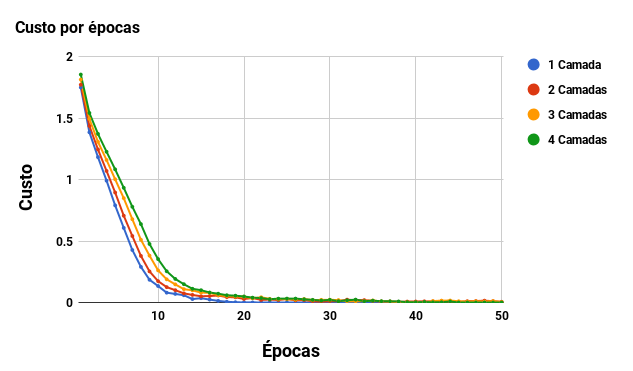
\includegraphics[scale=0.28]{Images/Loss.png}}
	}
	\caption{Custo por época das redes com diferentes números de camadas escondidas.}
	\label{fig:grafico}
\end{figure}

Podemos perceber que conforme o número de camadas cresce maior é o número de épocas necessárias. Além disso, o gráfico nos mostra que os modelos estão convergindo. Ou seja, o resultados não tendem melhorar muito com o aumento do número de épocas. Isso indica que para o treinamento de redes com mais camadas, como $3$ e $4$ camadas, é necessário um maior número de dados. A Tabela~\ref{tab:time} mostra o tempo que os experimentos levam em média por época, mostrando o motivo de épocas maiores que 100 não serem empregadas neste trabalho.

\begin{table}[h!]
	\centering
	\begin{tabular}{lcccc} \toprule
         & \multicolumn{4}{c}{\textbf{Tempo por época}} \\ \toprule
         \backslashbox{\textbf{GPU}}{\textbf{\emph{Nº Cam Esc}}}    & \emph{1}          & \emph{2}          & \emph{3}          & \emph{4}         \\ \toprule
         GeForce GTX 980 & 11s         & 15s         & 19s         & 23s \\
         GeForce GTX 1060 & 9s         & 12s         & 15s         & 18s \\  
         \toprule
	\end{tabular}
	\caption{Tempo dos experimentos por época.}
	\label{tab:time}
\end{table}

Considerando que todas as redes implementadas neste trabalho utilizam o \emph{framework} do Keras, a checagem de gradiente não se faz necessária, uma vez que sabe-se que a implementação do \emph{framework} está correta. Mesmo assim, houve a tentativa de implementar uma checagem do gradiente para cumprir os requisitos do trabalho. Porém, devido a restrições do Keras e a necessidade de mexer diretamente com as estruturas do Theano, a implementação acabou consumindo muito tempo e mostrou ter alto grau de complexidade. Assim, decidiu-se realizar outros experimentos pertinentes ao trabalho ao invés de finalizar a implementação do mesmo.

\subsection{Resultados dos melhores modelos na base de testes}

Esta seção tem como objetivo confirmar o resultados obtido com o melhor modelo encontrado para as redes neurais e regressão logística nos experimentos anteriores. Assim, o conjunto de teste foi utilizado para obter tais resultados e confirmar uma boa convergência do modelo também no conjunto de teste, ou seja, sem que haja \emph{overfitting}. Para os experimentos realizados com redes neurais, as funções de ativação \emph{relu} e \emph{softmax} foram utilizadas, variando o número de épocas entre $20$ e $100$. A Tabela~\ref{tab:result} mostra os resultados obtidos na base de teste.

\begin{table}[h!]
	\centering	
	\begin{tabular}{lccc} \toprule
		\textbf{Modelo} & \textbf{Nº Cam Esc} & \textbf{Épocas} & \textbf{Acurácia}    \\ \toprule 	
		Reg Logística (\emph{one-vs-all}) & - & - & 0.391 \\
		Reg Logística (Multinomial) & - & - & 0.402 \\  \toprule 
	    Rede Neural & 1 & 20  & 0.580 \\
   	    Rede Neural & 1 & 100 & \textbf{0.594} \\
	    Rede Neural & 2 & 20  & 0.586 \\
	    Rede Neural & 2 & 100 & 0.587 \\
	    Rede Neural & 3 & 50  & 0.585 \\
   	    Rede Neural & 4 & 50 &  0.568\\
	    
		\bottomrule      
	\end{tabular}
	\caption{Resultado dos modelos desenvolvidos no trabalho.}
	\label{tab:result}
\end{table}

Primeiramente os resultados mostram, como o esperado, que as regressões logísticas não são bons candidatos para resolver o problema, ambas obtiveram resultados bem inferiores aos outros modelos. Foi observado também que a rede com $4$ camadas apresentou a menor taxa de acurácia no conjunto de teste, como explicado  tem a necessidade de um maior número de dados para aprender.

A rede neural com $3$ camadas escondidas apresentou um resultado melhor do que o esperado, utilizando apenas $50$ épocas. Um dos motivos para essa melhora pode se dar por haver mais dados para o treinamento, considerando todo o conjunto de treinamento, quando antes considerava-se a validação cruzada. Há uma possibilidade desse aumento dos dados de treinamento ter proporcionado uma melhora na rede com três camadas.

E como era esperado os modelos com uma e duas camadas escondidas obtiveram resultados de acurácia melhores. O melhor resultado foi de $0.594$ de acurácia obtido pela rede com uma única camada escondida durante $100$ épocas. Redes com uma camada escondida convergem com menos facilidade para mínimos locais, comparado com redes com muitas camadas escondidas.

A melhora dos resultados em geral sobre os obtidos no processo de treinamento pode ser explicado pelo aumento do número de dados utilizados no treinamento, mostrando o quanto o número de dados importante para o processo. Tal melhora permite observar, também, que o modelo não apresentou \emph{overfitting} nos dados. A normalização realizada no pré-processamento dos dados teve significativa importância para tal questão.

Acredita-se que processos de gerar novos de dados para treinamento poderiam melhorar o resultado com redes de mais camadas escondidas e provavelmente ultrapassar o resultado obtido com a rede de só uma camada.

A Figura~\ref{fig:confusion} mostra a matriz de confusão normalizada para o modelo com o melhor resultado: 1 camada escondida, 100 épocas e funções de ativação \emph{relu} e \emph{softmax}.

\begin{figure}[!h]
	\centering
	{
		\setlength{\fboxsep}{1pt}
		\setlength{\fboxrule}{1pt}
		\fbox{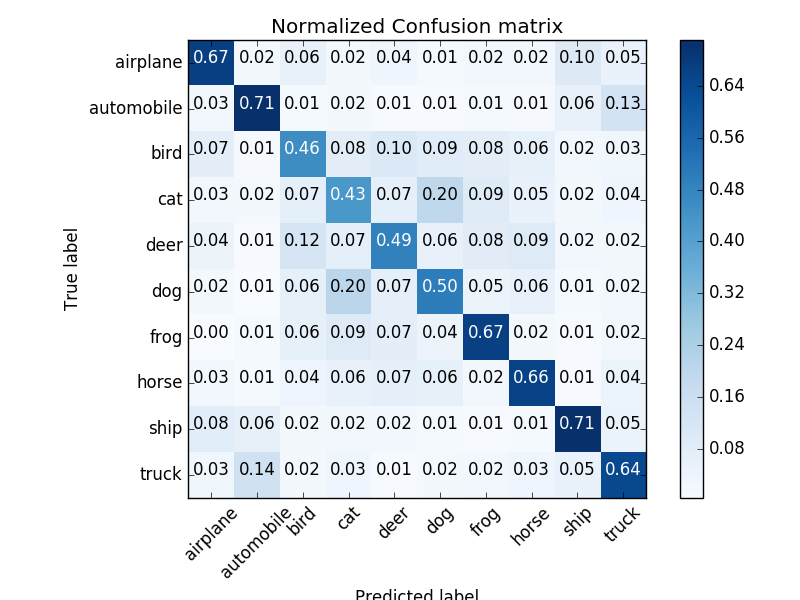
\includegraphics[scale=0.28]{Images/cm100epochs_norm.png}}
	}
	\caption{Matriz de confusão obtida considerando o melhor modelo no conjunto de test.}
	\label{fig:confusion}
\end{figure}

A matriz de confusão mostra que o modelo proposto é bom em reconhecer aeronaves, cavalos, carros e navios. Porém o mesmo tem muita dificuldade em reconhecer classes como ave, gato, cachorro e veado. O modelo confunde bastante cachorro e gato, assim como gatos e ave e caminhão e carros.

Pode-se perceber que todos as confusões feitas pelo sistema são relacionada a características similares, como por exemplo, cachorro e gato. Reforçando a necessidade de uma maior quantidade de dados para o processo de treinamento para poder utilizar redes mais profundas que aprendas informações mais complexas sobre as classes propostas nesse trabalho.

%\begin{thebibliography}{00}
%\bibitem{b1} Christopher M. Bishop. ``Pattern Recognition and Machine Learning''. Springer-Verlag New York, Inc., Secaucus, NJ, USA, 2006.
%\bibitem{b1} Aurélien Géron ``Hands-On Machine Learning with Scikit-Learn and TensorFlow
%Concepts, Tools, and Techniques to Build Intelligent Systems". O'Reilly Media, March 2017.
%\end{thebibliography}


\end{document}
